% Meld: the larger root becomes the first child of the smaller root.
% Editable source for this diagram. From this directory, regenerate with:
% latex -interaction=nonstopmode -halt-on-error pairing-heap-3.tex
% dvisvgm --no-fonts --exact --bbox=papersize --output=pairing-heap-3.svg pairing-heap-3.dvi
\documentclass[tikz,border=2pt]{standalone}
\usepackage{lmodern}
\usepackage{tikz}
\usetikzlibrary{arrows.meta,backgrounds,shapes.geometric,patterns}
\definecolor{linkred}{HTML}{B5240A}
\definecolor{noteBlue}{HTML}{0067A5}
\definecolor{softgreen}{HTML}{D8EAD0}
\definecolor{softpurple}{HTML}{D9D1E8}
\definecolor{softpink}{HTML}{F5CECF}
\definecolor{softyellow}{HTML}{FFF2C9}
\begin{document}
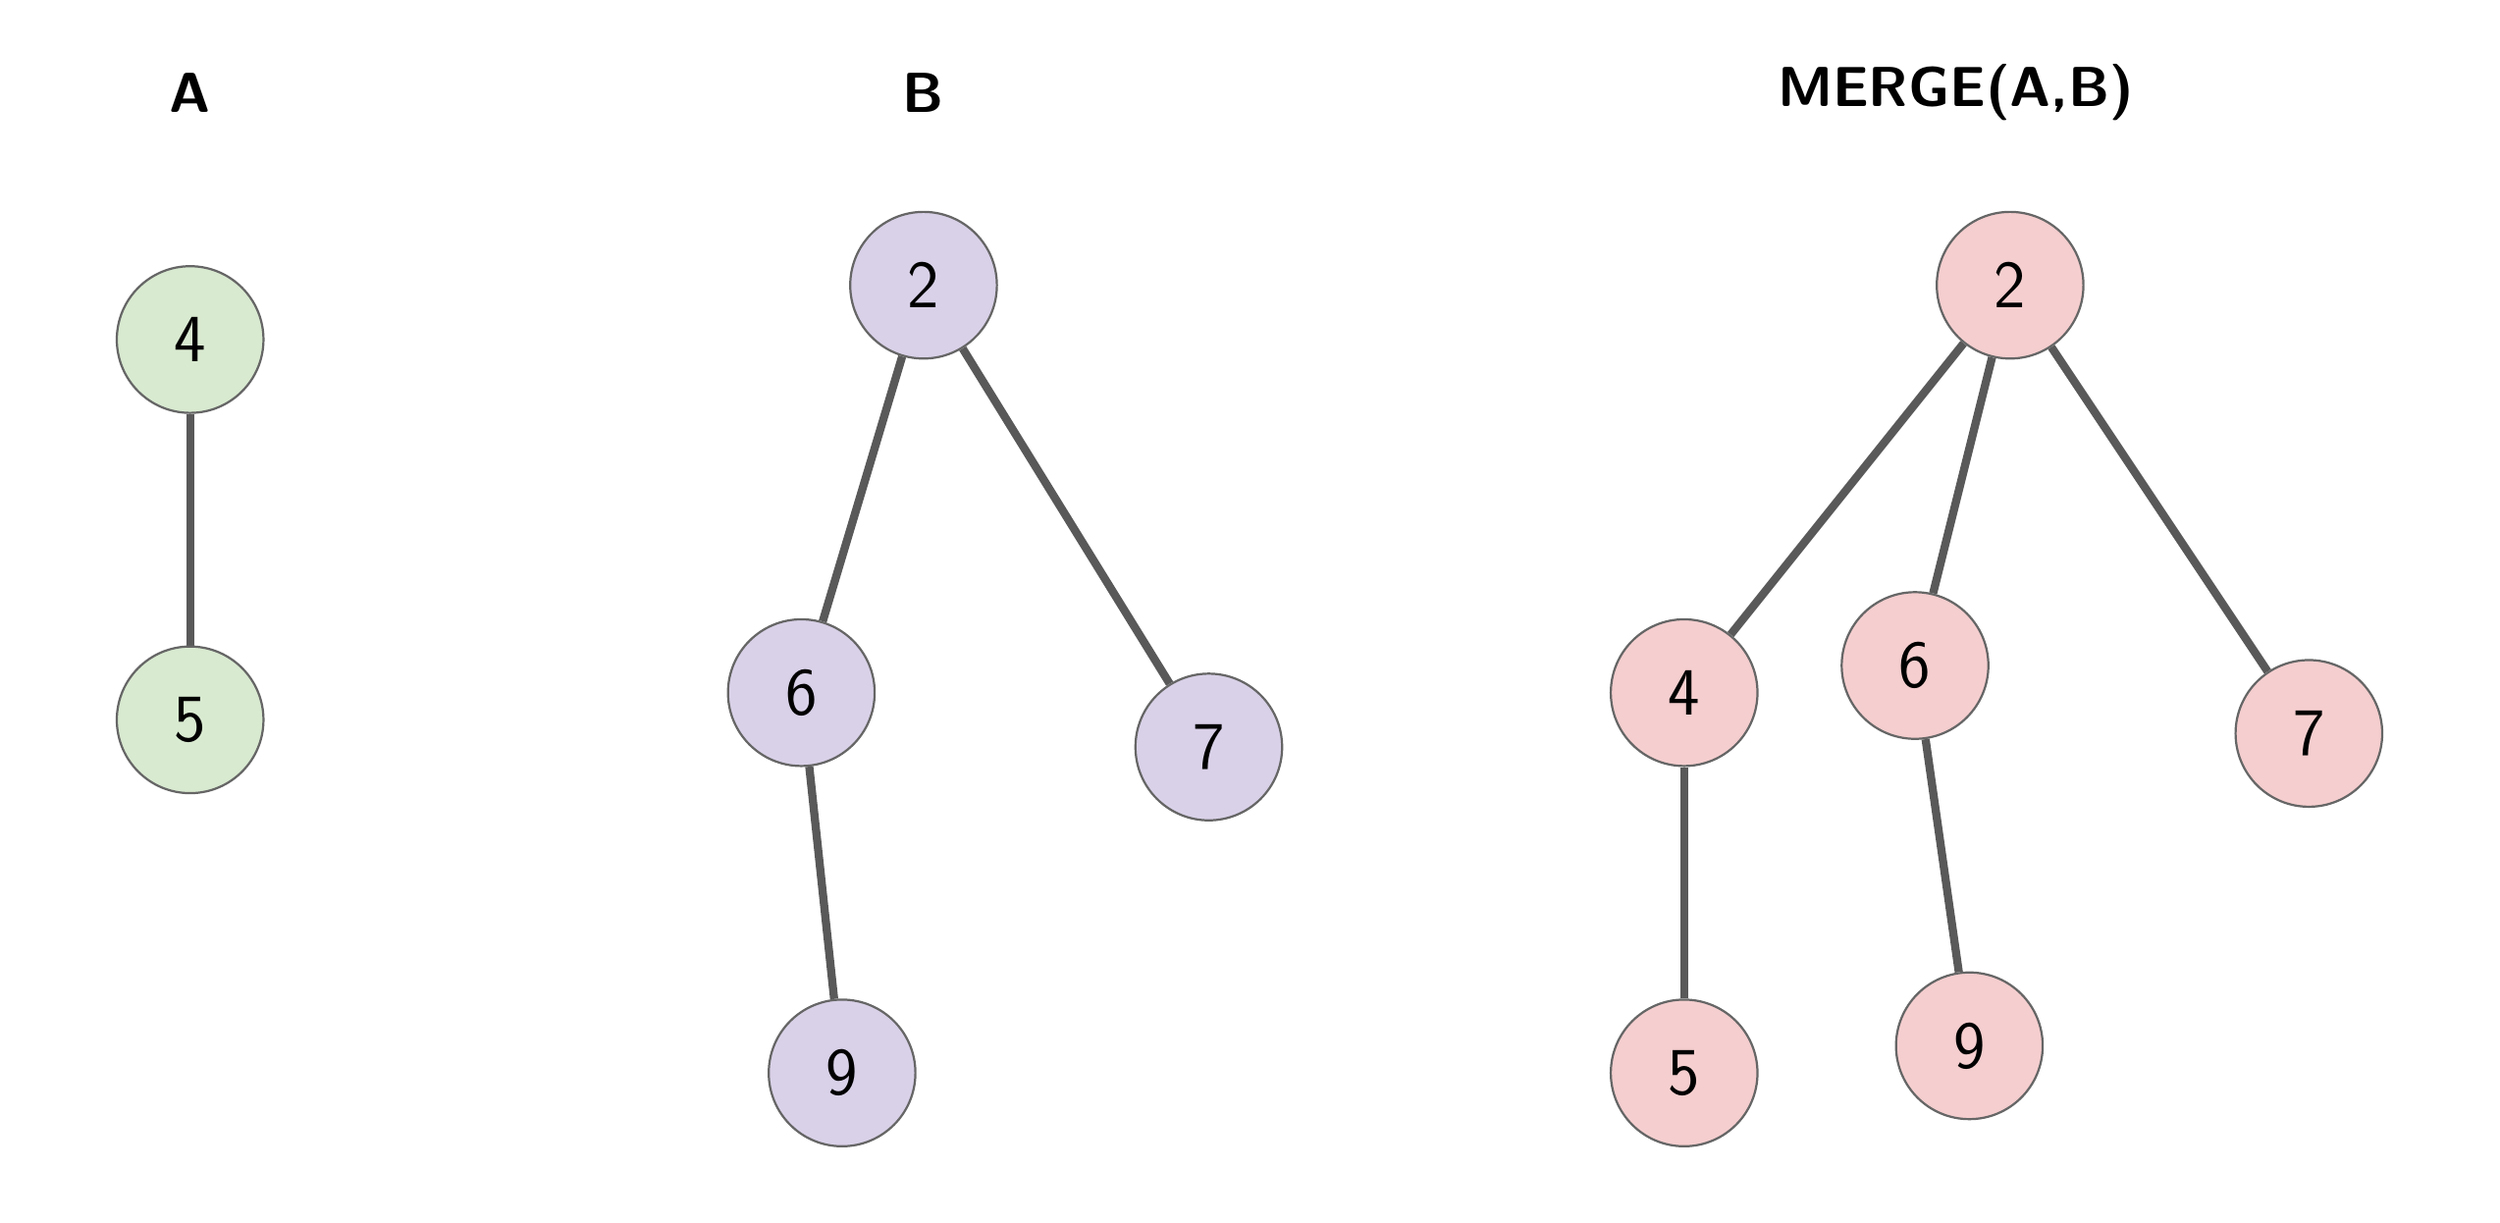
\begin{tikzpicture}[x=1pt,y=-1pt,>=Stealth,line cap=round,line join=round]
\path[use as bounding box] (0,0) rectangle (900,430);
\begin{scope}[on background layer]

\end{scope}
\node[circle,draw=black!60,fill=softgreen,text=black,minimum size=54pt,inner sep=0pt,line width=0.8pt,font=\sffamily\fontsize{25}{30}\selectfont] (a4) at (60,115) {4};
\node[circle,draw=black!60,fill=softgreen,text=black,minimum size=54pt,inner sep=0pt,line width=0.8pt,font=\sffamily\fontsize{25}{30}\selectfont] (a5) at (60,255) {5};
\node[circle,draw=black!60,fill=softpurple,text=black,minimum size=54pt,inner sep=0pt,line width=0.8pt,font=\sffamily\fontsize{25}{30}\selectfont] (b2) at (330,95) {2};
\node[circle,draw=black!60,fill=softpurple,text=black,minimum size=54pt,inner sep=0pt,line width=0.8pt,font=\sffamily\fontsize{25}{30}\selectfont] (b6) at (285,245) {6};
\node[circle,draw=black!60,fill=softpurple,text=black,minimum size=54pt,inner sep=0pt,line width=0.8pt,font=\sffamily\fontsize{25}{30}\selectfont] (b7) at (435,265) {7};
\node[circle,draw=black!60,fill=softpurple,text=black,minimum size=54pt,inner sep=0pt,line width=0.8pt,font=\sffamily\fontsize{25}{30}\selectfont] (b9) at (300,385) {9};
\node[circle,draw=black!60,fill=softpink,text=black,minimum size=54pt,inner sep=0pt,line width=0.8pt,font=\sffamily\fontsize{25}{30}\selectfont] (c2) at (730,95) {2};
\node[circle,draw=black!60,fill=softpink,text=black,minimum size=54pt,inner sep=0pt,line width=0.8pt,font=\sffamily\fontsize{25}{30}\selectfont] (c4) at (610,245) {4};
\node[circle,draw=black!60,fill=softpink,text=black,minimum size=54pt,inner sep=0pt,line width=0.8pt,font=\sffamily\fontsize{25}{30}\selectfont] (c6) at (695,235) {6};
\node[circle,draw=black!60,fill=softpink,text=black,minimum size=54pt,inner sep=0pt,line width=0.8pt,font=\sffamily\fontsize{25}{30}\selectfont] (c7) at (840,260) {7};
\node[circle,draw=black!60,fill=softpink,text=black,minimum size=54pt,inner sep=0pt,line width=0.8pt,font=\sffamily\fontsize{25}{30}\selectfont] (c5) at (610,385) {5};
\node[circle,draw=black!60,fill=softpink,text=black,minimum size=54pt,inner sep=0pt,line width=0.8pt,font=\sffamily\fontsize{25}{30}\selectfont] (c9) at (715,375) {9};
\begin{scope}[on background layer]
\draw[draw=black!65,line width=3pt] (a4) -- (a5);
\draw[draw=black!65,line width=3pt] (b2) -- (b6);
\draw[draw=black!65,line width=3pt] (b2) -- (b7);
\draw[draw=black!65,line width=3pt] (b6) -- (b9);
\draw[draw=black!65,line width=3pt] (c2) -- (c4);
\draw[draw=black!65,line width=3pt] (c2) -- (c6);
\draw[draw=black!65,line width=3pt] (c2) -- (c7);
\draw[draw=black!65,line width=3pt] (c4) -- (c5);
\draw[draw=black!65,line width=3pt] (c6) -- (c9);
\end{scope}
\node[anchor=center,text=black,font=\sffamily\fontsize{25}{30}\selectfont,font=\sffamily\bfseries\fontsize{22}{26}\selectfont] at (60,24) {A};
\node[anchor=center,text=black,font=\sffamily\fontsize{25}{30}\selectfont,font=\sffamily\bfseries\fontsize{22}{26}\selectfont] at (330,24) {B};
\node[anchor=center,text=black,font=\sffamily\fontsize{20}{24}\selectfont,font=\sffamily\bfseries\fontsize{22}{26}\selectfont] at (710,24) {MERGE(A,B)};
\end{tikzpicture}
\end{document}
